\documentclass[a4paper]{jpconf}
\usepackage{graphicx}
\usepackage{fixltx2e}

\graphicspath{{pics/}}

\newcommand{\dd}[1]{\mathrm{d}#1}

\setlength\intextsep{1mm}

%\bibliographystyle{iopart-num}
%\usepackage{citesort}

\begin{document}
\title{A Vision and GPS Based System for Autonomous Precision Vertical Landing of UAV Quadcopter}

\author{A S Priambodo\textsuperscript{1}, F Arifin\textsuperscript{2}, A Nasuha\textsuperscript{3}, Muslikhin\textsuperscript{4}, A Winursito\textsuperscript{5}}

\address{\textsuperscript{1,2,3,4,5}Department of Electronics and Informatics Engineering of Education, Engineering Faculty, Universitas Negeri Yogyakarta, Indonesia}

\ead{ardyseto@uny.ac.id}

\begin{abstract}
    This research aims to develop an algorithm for the precision vertical landing process on a quadcopter using GPS sensors and computer vision. This research consists of 2 main parts: GPS-based control used by the quadcopter to return to the home area and computer vision-based control in the form of ArUco marker detection, which is used by the quadcopter in order to land precisely. Detection of the ArUco marker that is used goes through 2 stages: the application of threshold and ratio and the process of calculating the black and white area, which can then be searched for four corners of the marker. The algorithm designed works well on the Webots simulation program with mid-computer specifications. The ArUco marker detection process is fast and reliable, so it does not overload the processor unit so that the simulation process can run well. From 30 tests with different initial positions, the average error of the landing position of the quadcopter at coordinate X is 0.02 meters, and coordinates Y is 0.03 meters. All test results show that the quadcopter can land inside the landing pad area without any parts coming out.\\

    \noindent{\it Keywords\/}: \it Quadcopter, GPS, Computer-Vision, Precision Landing, ArUco Marker

\end{abstract}

\section{Introduction}
Unmanned Aerial Vehicle (UAVs) or Drones is a topic of great interest to researchers now. A drone can do much work. In agriculture, drones are used as sprinklers of liquid fertilizer and observation of crops from the air\cite{ref1}. Drones are used as spies from the air in the military field\cite{ref2}. In the safety field, drones are used for surveillance in disaster areas\cite{ref3}. The quadcopter is one type of UAV that is widely developed because it has the advantage of being able to take off and land vertically. The quadcopter consists of four rotors that rotate the propellers to get lifts. Because the quadcopter can take off and land vertically, the required take-off area is minimal. In addition to these advantages, the quadcopter also can hover in the air.

There are various types of UAVs, namely fixed wing, rotary wing and hybrid fixed and rotary wing. In comparison, the rotary wing consists of 2 types: single rotor and multirotor. The hybrid and rotary wing UAV can take off and land vertically, so they do not require a large area. The selection of the type of UAV depends on the task and area to be completed. Multirotor has many advantages such as more agile manoeuvrability, ability to hover in the air, with a certain size, it can fly indoors, take off and land vertically and has a relatively simple frame design compared to other types\cite{ref4}. Multirotor also has disadvantages, namely limited flight time, which causes relatively small cruising area and limited carrying capacity. The multirotor that is widely developed is the quadcopter or quadrotor type. The quadcopter is a multirotor with 4 motors driving the propellers to generate lift. The quadcopter can be configured to be type X or H.

In general, flying vehicles' flight actions are based on GPS sensors\cite{ref5}. A global positioning system (GPS) is an electronic device that can be used for navigation\cite{ref6}. GPS provides latitude, longitude and altitude values as a reference from the UAV so that the UAV can fly to a certain point based on that reference. GPS on UAVs, especially quadcopters, is also used to get the take-off location and later used as a landing point. However, the GPS does not provide accurate values in some conditions and environments, so the landing becomes imprecise. In limited applications where the take-off and landing places are very narrow, this is a challenge, so we cannot just rely on GPS to find out the location of the landing point\cite{ref7}.

Manually landing a quadcopter usually has difficulties. For example, pilots find it difficult to gradually reduce the quadcopter's altitude and land smoothly and accurately at precise locations. Automatic landing using GPS is a method to facilitate the quadcopter land smoothly and accurately. However, in particular area and time conditions, the GPS accurateness becomes less good and causes the quadcopter not to land in the accurately determined area\cite{ref8}. In this paper, we propose a new automatic landing method based on GPS and computer vision so that the quadcopter can land precisely in the specified area. The take-off and landing area used in this study is an ArUco marker. Improved landing accuracy, safety and reliability are the advantages of our proposed method.

\section{Methodology}
\subsection{Quadcopter Model}
A quadcopter is a type of flying vehicle which has four motors used to rotate the propeller. The propeller's rotation here will generate lift to raise the quadcopter. Adjusting the speed on each quadcopter motor can perform roll, pitch, yaw or vertical movements. Quadcopters with X configuration consist of front right, rear right, rear left, and front left motors, usually numbered 1,2,3 and 4. Quadcopters with an X configuration of 1,3 and 2,4 propeller pairs rotate in opposite directions, eliminating momentum and not requiring a tail rotor for counterbalance. Besides, this research uses an X configuration quadcopter because it has better stability than the + configuration.

The roll movement is influenced by the speed of the right part (1,2) and left part(3,4) motors. Pitch movement is affected by the speed of the front part (1,4) and rear part (2,3) motors. Yaw movement is influenced by combination of motors 1,3 and 2,4. The speed of the four motors on the quadcopter influences the vertical movement. The illustration of the quadcopter movement can be seen in Figure 1.

\begin{figure}[h]
    \centering
    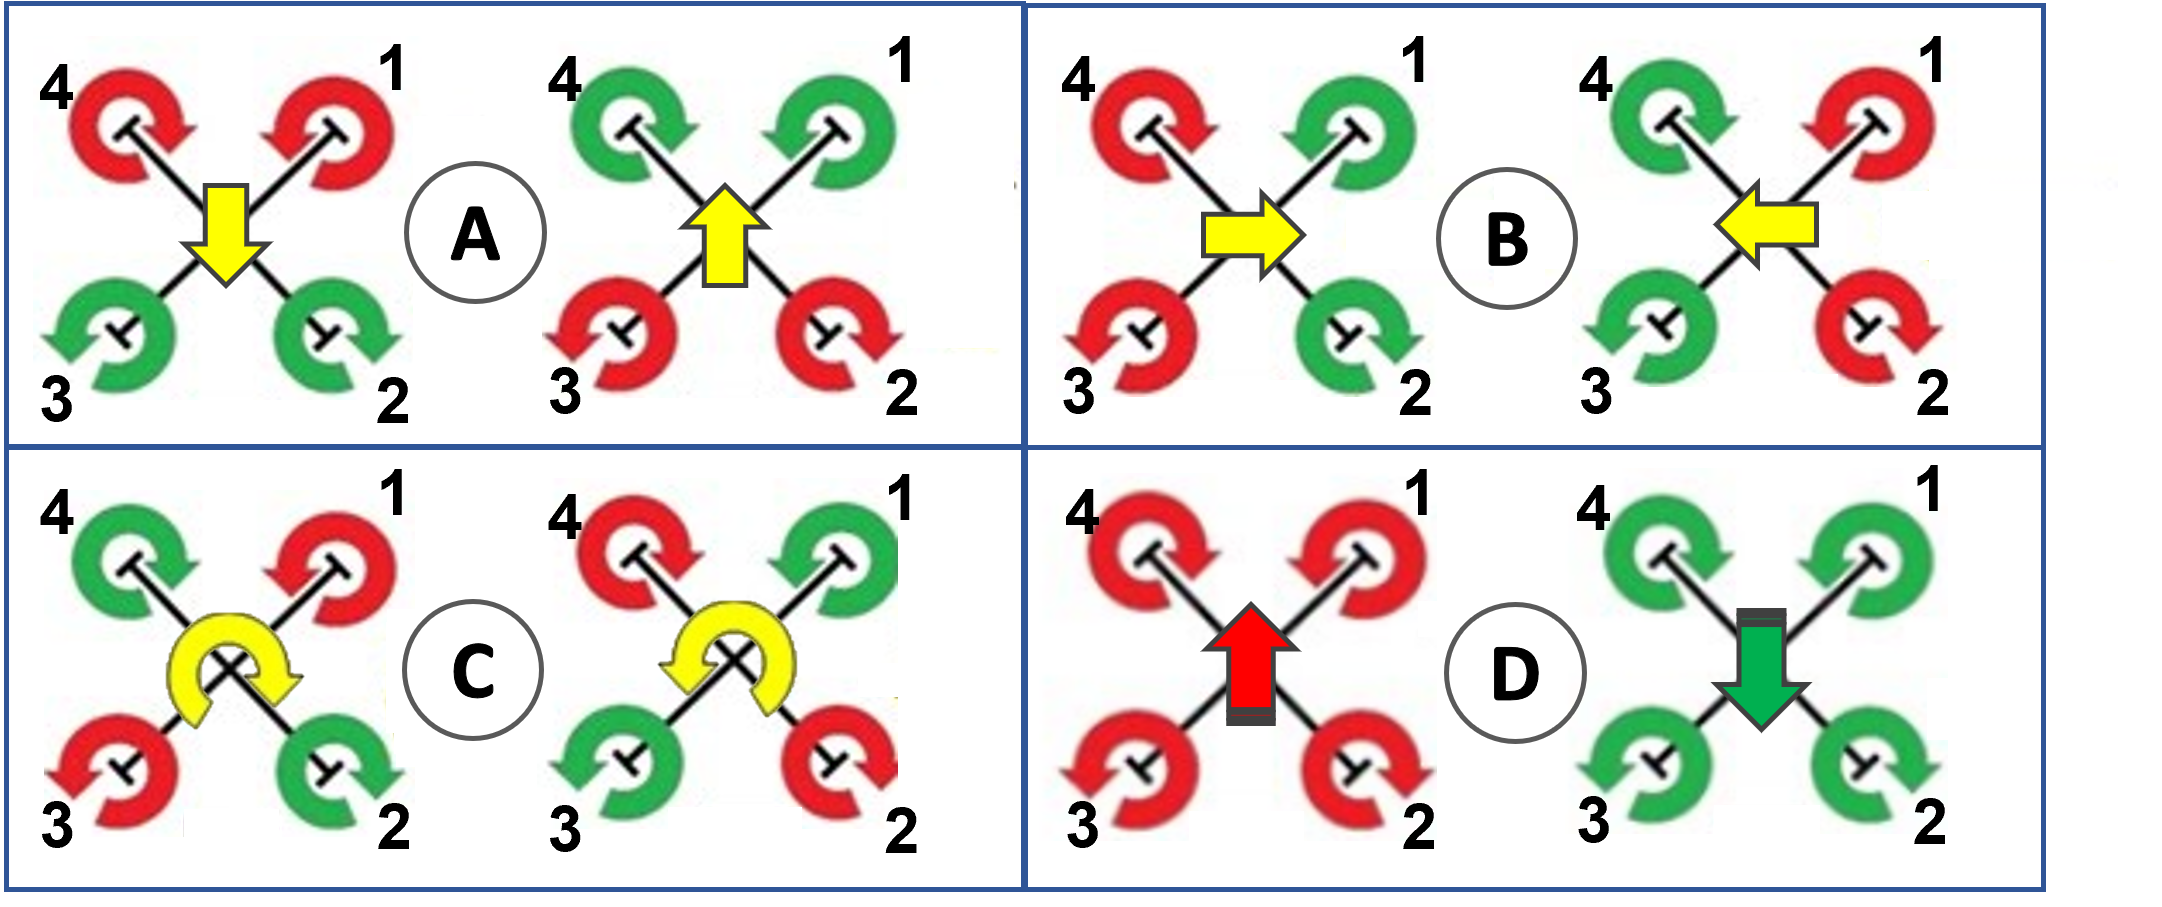
\includegraphics[width=20pc]{quadcopter-basic-movement.png}
    \caption{\label{label}Quadcopter Basic Movement: (A)Pitch (B)Roll (C)Yaw (D)Vertical Movement (the red color means faster than green)}
\end{figure}

Based on rotational and translational movements, a quadcopter mathematical model can be derived for 6-DOF using the Newton-Euler technique. Using this approach, the 6-DOF were deduced show in equation 1-6\cite{ref9}.

\begin{equation}
    \ddot{\phi}=\dot{\theta}\dot{\psi}\left ( \frac{I_{y}-I_{z}}{I_{x}} \right )-\frac{J_{r}}{I_{x}}\dot{\theta}\Omega+\frac{l}{I_{x}}U_{2}
\end{equation}

\begin{equation}
    \ddot{\theta}=\dot{\phi}\dot{\psi}\left ( \frac{I_{z}-I_{x}}{I_{y}} \right )-\frac{J_{r}}{I_{y}}\dot{\phi}\Omega+\frac{l}{I_{y}}U_{3}
\end{equation}

\begin{equation}
    \ddot{\psi}=\dot{\phi}\dot{\theta}\left ( \frac{I_{x}-I_{y}}{I_{z}} \right )+\frac{l}{I_{z}}U_{4}
\end{equation}

\begin{equation}
    \ddot{x}=(cos\phi sin\theta cos\psi + sin\phi sin\psi)\frac{U_{1}}{m}
\end{equation}

\begin{equation}
    \ddot{y}=(cos\phi sin\theta cos\psi - sin\phi sin\psi)\frac{U_{1}}{m}
\end{equation}

\begin{equation}
    \ddot{z}=-g+(cos\phi cos\theta)\frac{U_{1}}{m}
\end{equation}

\subsection{Vision-Based Landing}
Several artificial fiducial marking systems exist April-Tags, ArUco, and ARToolKit\cite{ref10}. With this comparison, ArUco detection can detect markers quickly and reliably\cite{ref11}. Therefore, the ArUco marker was used as a landing pad in this study. The ArUco marker is a synthetic square marker composed of a wide black border and an inner binary matrix that defines its identifier. Black border for fast image detection and binary codification enables and application of detection and error techniques. The marker's size determines the internal matrix's size; for example, the 4x4 marker size consists of 16 bits. ArUco markers generated for landing pads have specifications, as shown in Table 1. We can create ArUco markers using python and OpenCV or through websites that provide ArUco Generator services. The generated marker is an image file in PNG or JPG format shows in Figure 2.

\begin{table}[h]
    \centering
    \caption{\label{opt}Parameter of ArUco marker used}
    \begin{tabular}{@{}*{7}{l}}
        \br
        Parameter        & Value                    \\
        \mr
        Dictionary       & 6x6 (50, 100, 250, 1000) \\
        Marker ID        & 1                        \\
        Marker size (mm) & 100                      \\
        \br
    \end{tabular}
\end{table}

By using OpenCV in the ArUco marker detection process, we will get two values, namely (1) the position of the four corners of the marker; (2) the id of the marker. In this study, what is needed is the position of the four corners so that the midpoint of the marker can be calculated, which can then be calculated for the error in the position of the camera's centre. The marker detection process consists of several steps\cite{ref12}. The first step is to apply an adaptive threshold by calculating the average value of the surrounding pixels of a given pixel. This way, all the contours in the image are expected to be found, and then the non-square shapes are filtered. The next step is to extract the marker bits in the picture. The first perspective transformation is applied to get the marker in canonical form. Then the canonical image is subjected to a threshold process using otsu to separate the white and black bits. The image is divided into cells according to marker size and border size.

%\begin{figure}[h]
%    \centering
%    \includegraphics[width=6pc]{ArUco-land.png}\hspace{2pc}%
%    \begin{minipage}[b]{14pc}\caption{\label{label}ArUco marker used in this research}
%    \end{minipage}
%\end{figure}

The number of black and white pixels in each cell is then counted to determine whether it includes black or white bits. The final step is to compare with a specific dictionary. The results obtained are the position of the four corners and the id value of the marker. After getting the position of the four corners of the marker, the centre of the marker can be calculated, which can later be used to calculate the position of the X and Y errors by comparing with the midpoint of the camera capture, as shown in Figure 2. The X and Y position error values will be used to adjust the roll and pitch angle of the quadcopter to correct its position according to the desired set point.

\begin{figure}[h]
    \centering
    \includegraphics[width=10pc]{camera-capture-ArUco.png}\hspace{2pc}%
    \begin{minipage}[b]{14pc}\caption{\label{label}Calculation X and Y position error based on detection of ArUco Marker}
    \end{minipage}
\end{figure}

\subsection{Proposed Landing Control}
GPS is a Global Positioning System, a tool or system that can use to inform users that they are (globally) on the surface of the earth based on satellites. GPS is installed on the flight controller so the flight controller can find out where the quadcopter is. The flight controller can store the take-off position so that, theoretically, the quadcopter can land in the take-off area. In addition, GPS can also function as flying navigation at specific coordinate points.

\begin{figure}[h]
    \centering
    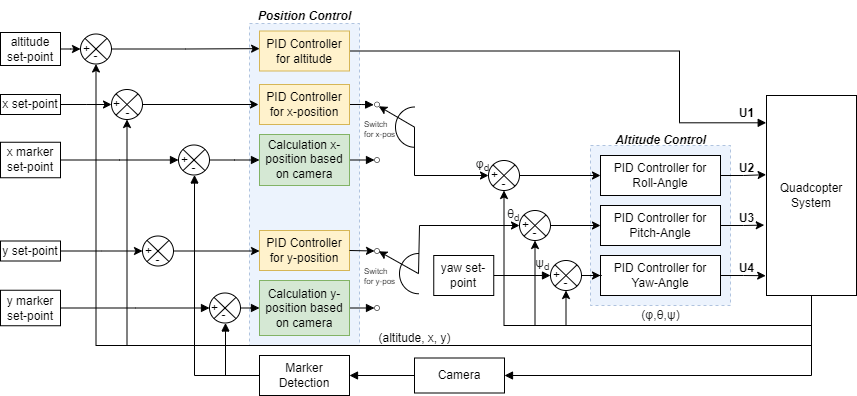
\includegraphics[width=30pc]{block-diagram-controller.png}
    \caption{\label{label}Block Diagram of Proposed Controller}
\end{figure}

There are two control loops designed, namely attitude control and position control. Position control is in charge of adjusting the translational position of the quadcopter so that it is right at specific coordinates and altitudes. The output of the position control is the set point values for the roll and pitch angles. The roll and pitch set point values will be input for attitude control so that the quadcopter will move to follow the set points from a predetermined position. The block diagram used in this control proposal is shown in Figure 3. The control system used in this proposal is a PID control system known to be reliable in correcting various systems. The PID control system consists of 3 components: proportional control, integral control, and derivative control. The equation of the PID control system is shown in equation 7\cite{ref13}.

\begin{equation}
    u(t)=K_{p}e(t)+K_{i}\int_{0}^{t}e(t)dt+K_{d}\frac{de(t)}{dt}
\end{equation}

It has been mentioned that GPS has shortcomings, so there is an additional camera used to detect the ArUco marker, which functions as a landing pad. The reference from the position control will switch from GPS to the estimated position based on the camera when the quadcopter camera detects the marker. That way, the quadcopter will position exactly above the marker, and the process of lowering the height is carried out slowly until the quadcopter touches the ground. The proposed control running the algorithm is shown in Figure 4.

\begin{figure}[h]
    \centering
    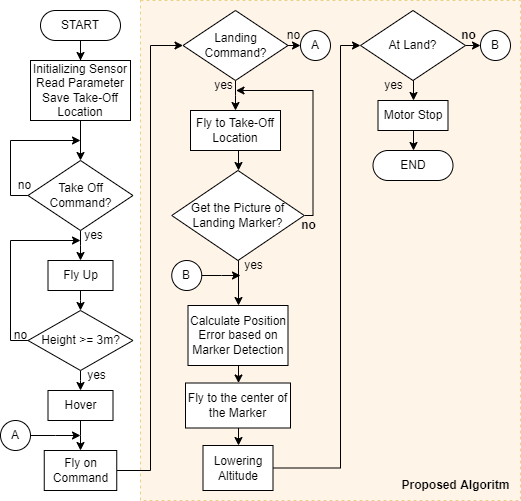
\includegraphics[width=20pc]{flowchart-proposed-algorithm.png}
    \caption{\label{label}Proposed Flowchart of Vision and GPS Based System for Vertical Landing Quadcopter}
\end{figure}

\subsection{Simulation Environment}
Webots is an application or software developed by the Swiss Federal Institute of Technology that serves to create models, programs, and simulations of a robot. Using webots, we can design or design and develop programs that will run robots in an artificial environment. This application was first developed in 1996 by Dr Oliver Michael. Then in 1998, it was developed again by Cyberbotics Ltd. as proprietary licensed software. Thanks to Cyberbotics Ltd in 2018, made webots an open source application so that it is easy to use and its development becomes more available. Webots can be installed on Windows, Mac OS and Linux (Ubuntu) operating systems.

Webots provides many components in the form of robots, sensors, actuators and other objects such as humans, animals, boxes and many other things that we can use in an artificial environment. In addition, we can also create our objects through 3D CAD applications.The programming languages supported by webots also vary, namely Matlab, C/C++, Python, Java and ROS. This study uses a DJI Mavic 2 Pro drone shows in Figure 5, in which the proposed controller will simulate a yard environment consisting of several objects such as houses, cars, roads, and many trees. Webots version used in theis research is R2022a. The landing pad used to search at the top is displayed with the ArUco marker, which the quadcopter will later recognize as the area for landing. DJI Mavic 2 Pro consists of several sensors such as an accelerometer, gyroscope, barometer, compass and GPS that we can access through the program. In the webots, we can adjust the speed of each motor so that when hovering, it must be designed first before designing before landing. The stability of the hover quadcopter is essential because, in the precision landing process, the quadcopter must be able to lower its altitude without any change in position. The webots simulation program is run on a computer with the specifications listed in Table 2.

\begin{table}[h]
    \centering
    \caption{\label{opt}Computer Spesification}
    \begin{tabular}{@{}*{7}{l}}
        \br
        Component        & Description     \\
        \mr
        CPU              & Intel i5 12400F \\
        RAM              & 2x8GBs          \\
        GPU              & RTX 3060 12GB   \\
        Storage          & SSD NVMe Gen4x  \\
        Operating System & Ubuntu 20.04    \\
        \br
    \end{tabular}
\end{table}

\begin{figure}[h]
    \centering
    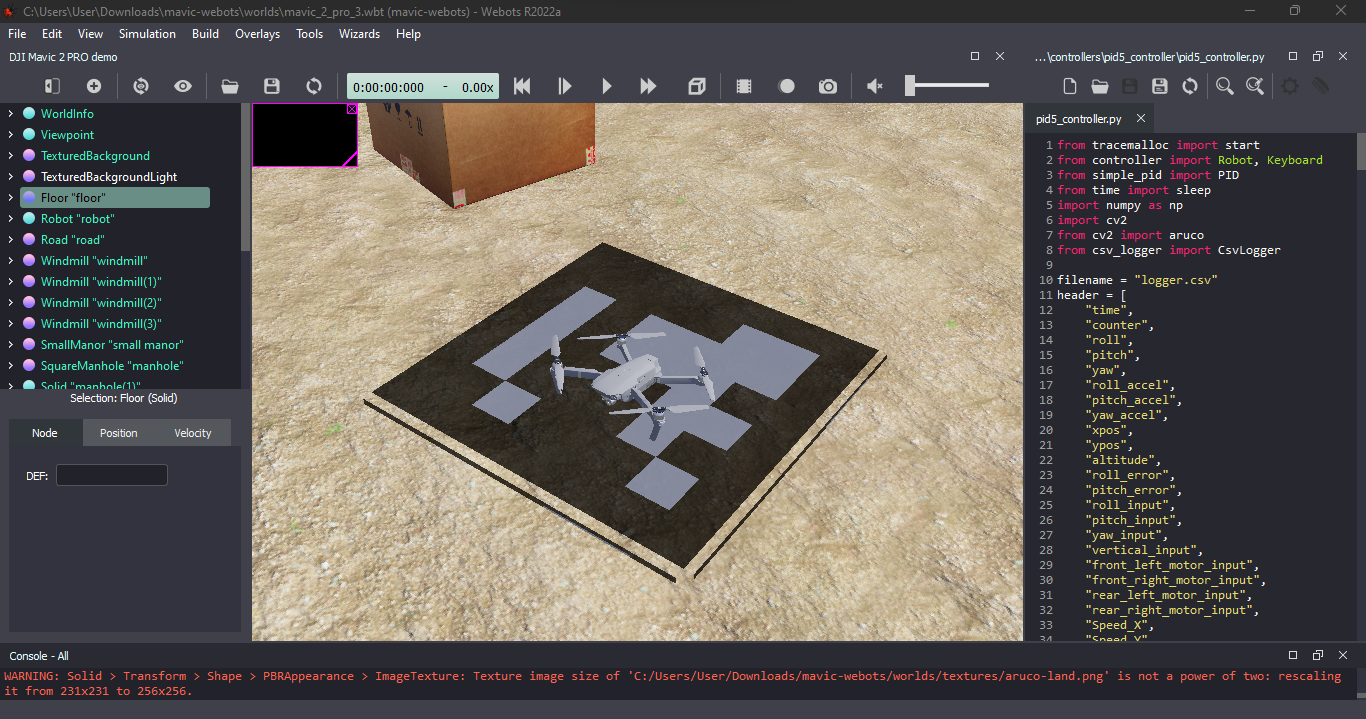
\includegraphics[width=30pc]{webots-dji-mavic-2pro.png}
    \caption{\label{label}DJI Mavic 2 Pro in Webots Environment}
\end{figure}

\section{Result and Discussion}
This section will show the results of testing the proposed control system—several tests on the ArUco marker detection section and overall system testing involving GPS and Computer Vision.

\subsection{Marker Detection}
The ArUco marker detection test is carried out by positioning the quadcopter at several X and Y positions and heights, as shown in Figure 6. To make it easier to observe, the roll, pitch, and yaw angle data, as well as the X, Y, and altitude positions, are displayed on the simulation screen of the webots. Before testing, the gimbal camera must be directed downwards, and there is a control mechanism that makes the camera direction always perpendicular to the ground so that it is hoped that the marker is caught. The camera is in a perfect square shape. Shown in figure 7 and 8, obtained at the height of 2.17 meters is the minimum height that the quadcopter must reach for the camera to detect the presence of a marker. In comparison, the maximum value is 29.85 meters. Beyond this altitude value, the marker cannot be detected, so the quadcopter is set when returning to home mode at 20 meters. The results of this height measurement are shown in Figures 8 and 9, where the marker will be overlaid with a transparent green box.

\begin{figure}[h]
    \centering
    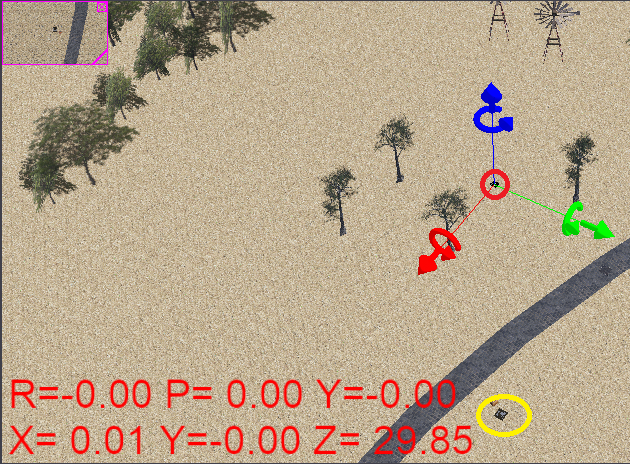
\includegraphics[width=20pc]{marker-detection-testing-edit.png}
    \caption{\label{label}Marker detecion testing in Webots. There is information about the translational and rotational position of the quadcopter which is displayed in red font. The quadcopter is marked with a red circle and the ArUco marker is marked with an yellow circle.}
\end{figure}

\begin{figure}[h]
    \centering
    \begin{minipage}{15pc}
        \includegraphics[width=16pc]{ArUco-at-2m.png}
        \caption{\label{label}Minimum range of ArUco marker detection at a distance of 2.17 meters}
    \end{minipage}\hspace{2pc}%
    \begin{minipage}{15pc}
        \includegraphics[width=16pc]{ArUco-at-29m.png}
        \caption{\label{label}Maximal range of ArUco marker detection at a distance of 29.85 meters}
    \end{minipage}
\end{figure}

\subsection{Precision Landing}
Overall, testing was carried out after marker detection worked well. Initially, the quadcopter was flown randomly in both X, Y and altitude positions. In this test, the initial position of the quadcopter is X = -11.9m which means its position is towards the back of the home, Y = -8.6m which means its position is to the right of the home, and the initial height is 16.48m. After the quadcopter is in the initial place, the return to home mode is activated. Autonomously the quadcopter will rise to a safe height of 20 meters. After the altitude is reached, the X and Y positions are corrected based on the GPS sensor so that the quadcopter will move towards the landing pad. With a height of 20 meters, the marker will be easily visible; as soon as it is detected, the position reference is replaced on the detection results of the ArUco marker. The quadcopter will then lock its position right above the landing pad so that the quadcopter lowers its height slowly until it hits the landing pad. When the quadcopter has landed perfectly, all the motors will stop turning. Figure 9 shows that this process is going well, and the quadcopter can land perfectly on the landing pad. This can be seen in Figure 10.

Testing at this stage was carried out several times with different initial positions. From 30 times of testing, the error rate of landing position based on GPS reference at X coordinates is 0.02 meters on average, and Y coordinates are 0.03 meters. All test results show that the quadcopter can land inside the landing pad area without any parts coming out.

\begin{figure}[h]
    \centering
    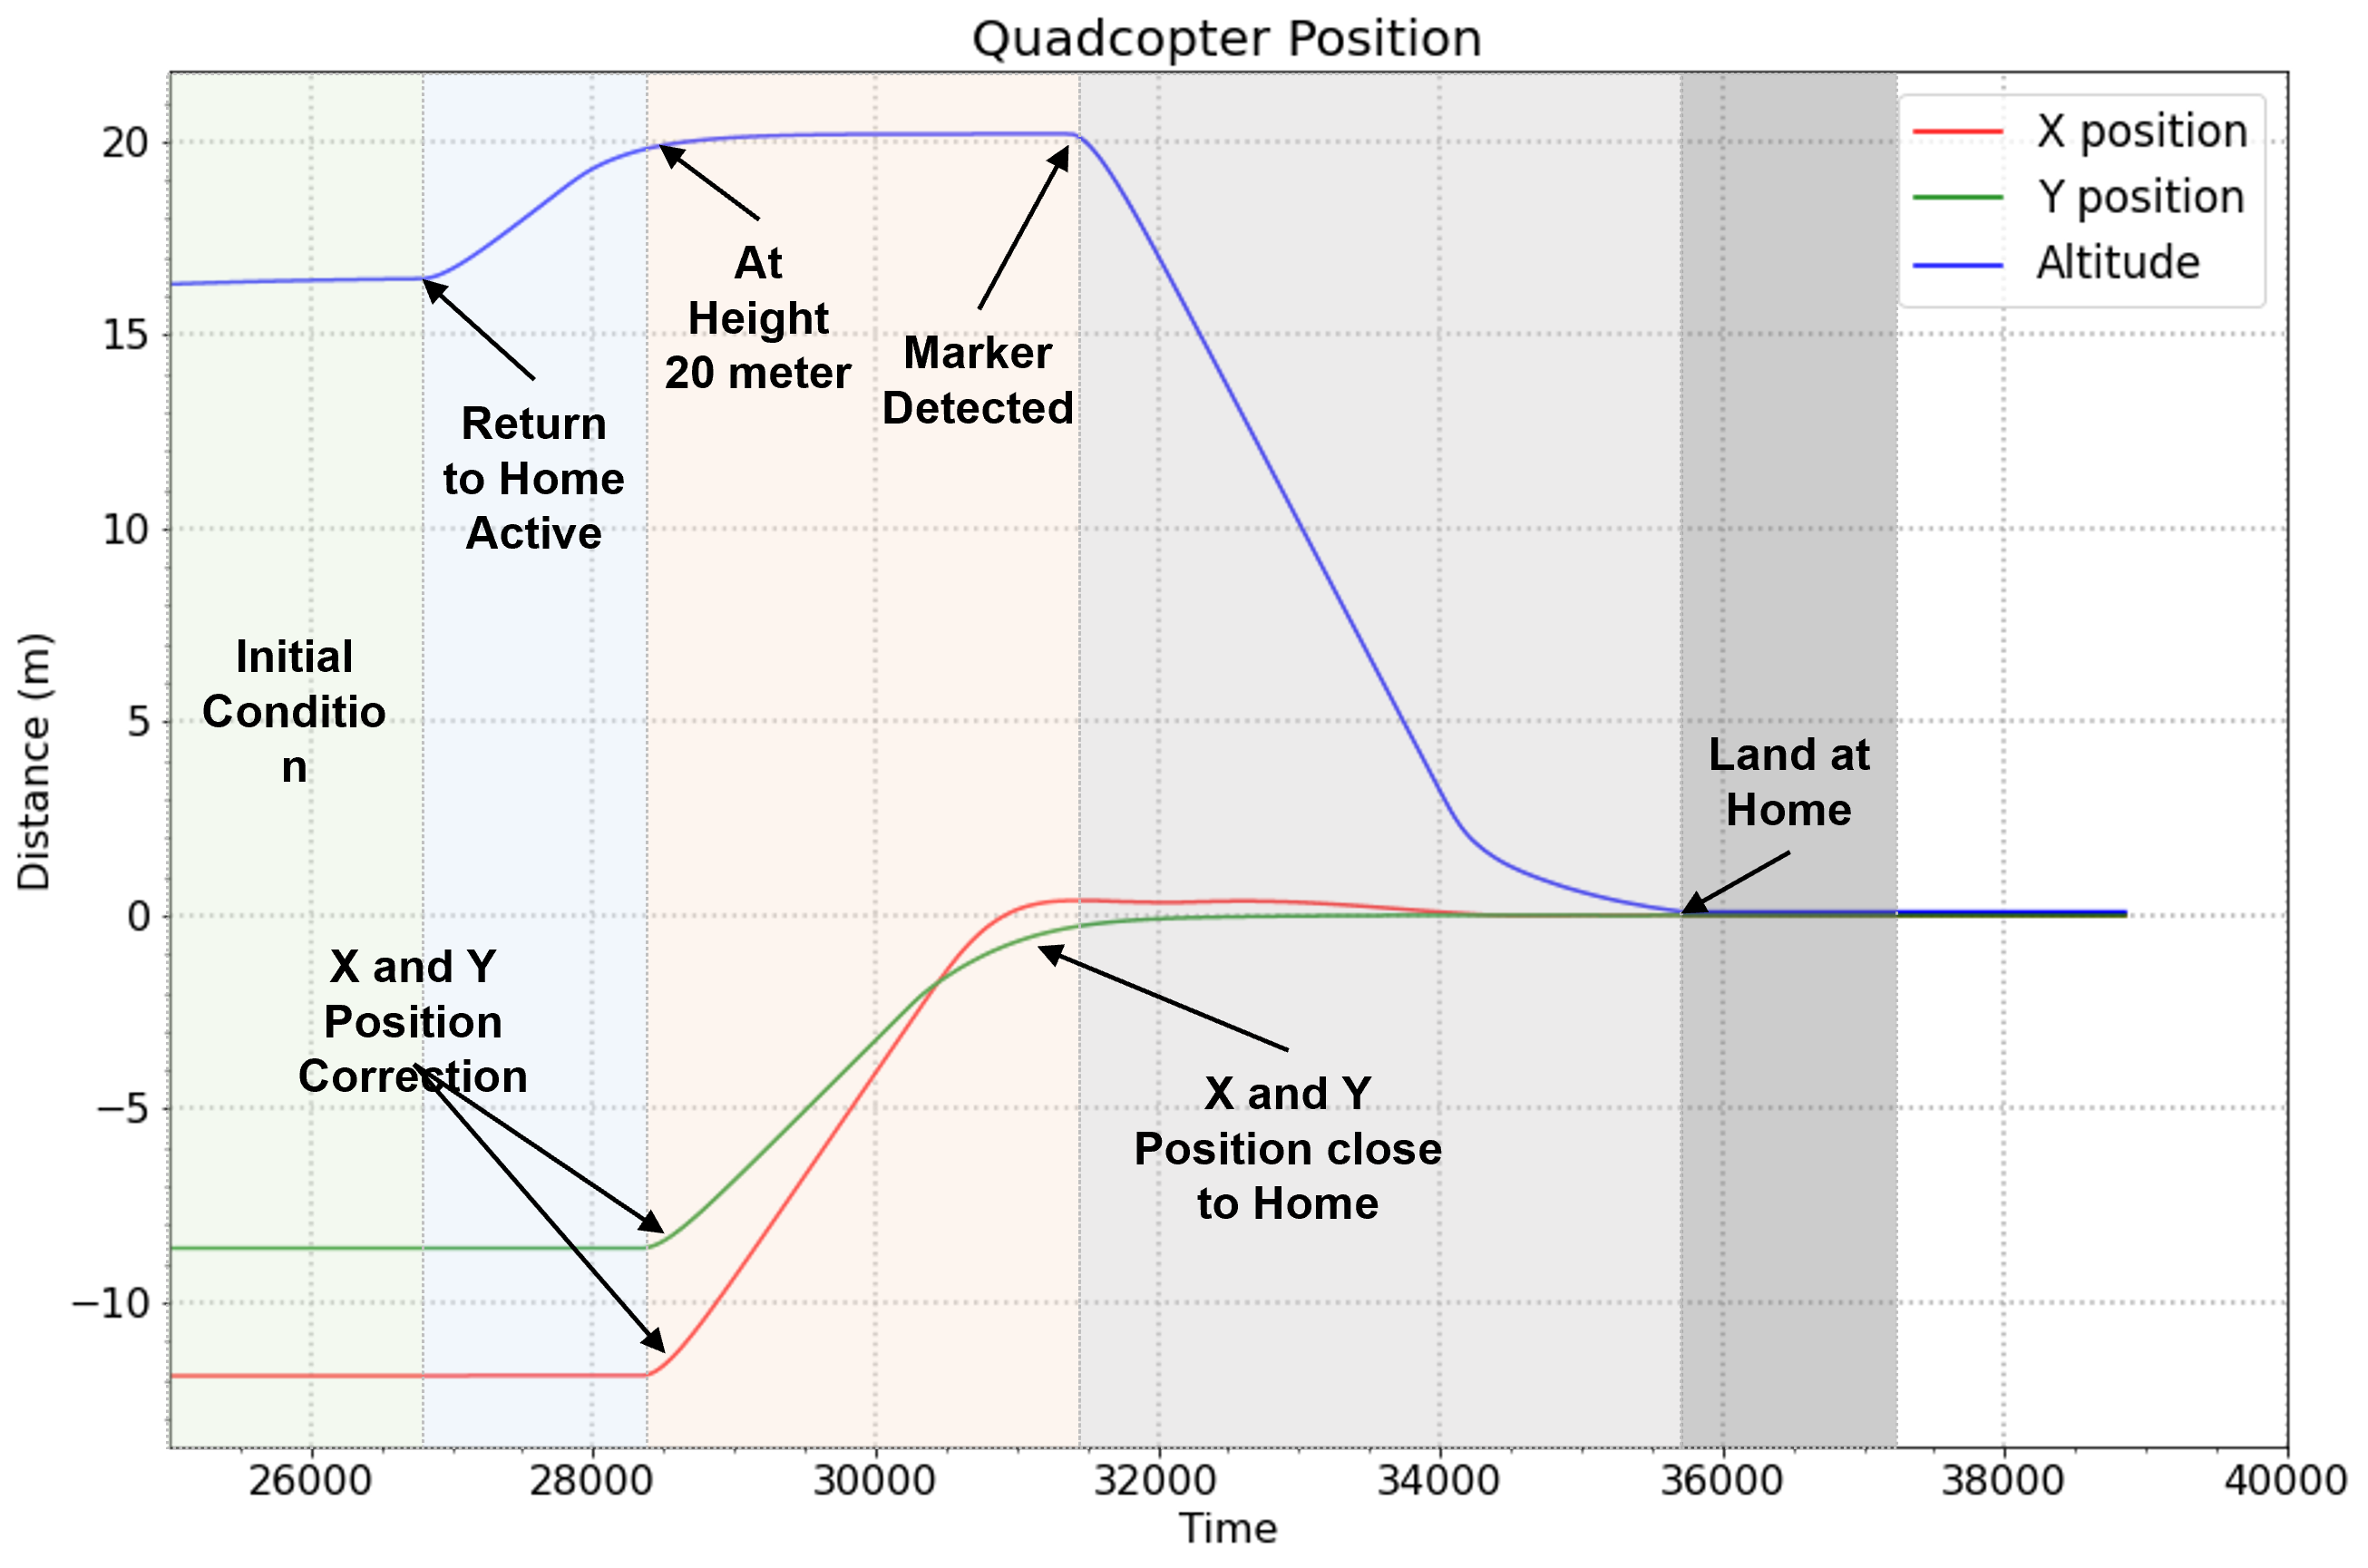
\includegraphics[width=28pc]{graph-response-position-edited.png}
    \caption{\label{label}X, Y Position, and Altitude of quadcopter in Autonomous Vertical Landing}
\end{figure}

\begin{figure}[h]
    \centering
    \includegraphics[width=32pc]{process-of-landing.png}
    \caption{\label{label}Process of Autonomous Vertical Landing: (a) Intial Position of Quadcopter; (b) Return to Home activated; (c) Position Correction based on GPS; (d) Marker detected; (e) Marker at Center of Camera Capture; (f) decrease height of quadcopter, closed to landing pad; (g) landing successful at landing pad}
\end{figure}

\section{Conclusion}
The test results show that the combination of GPS and computer vision in the implementation of precision landing on a quadcopter can work well and as expected. The quadcopter can land right on the landing pad without the help of GPS. The role of GPS here is only when the quadcopter goes to the home point, and when the marker has been detected, all landing operations will use the reference from the marker detection. The detection using computer vision on ArUco marker objects is fast and reliable, so the processor unit does not need to work more during the detection process. The obstacle that may be faced when implemented in real life is that it requires a camera gimbal that can be adjusted perpendicular to the ground so that the camera captures are perfect.

\section*{Acknowledgments}
This work was supported by the Group Research Research Grant for the BEAIS Research Group in 2021 which was funded by DIPA Yogyakarta State University, Indonesia.

\section*{References}
\begin{thebibliography}{12}
    \bibitem{ref1} Jain M, Bajwa M S and Kumar H 2022 Agriculture Assistant for Crop Prediction and Farming Selection Using Machine Learning Model with Real-Time Data Using Imaging Through UAV Drone Emergent Converging Technologies and Biomedical Systems ed N Marriwala, C C Tripathi, S Jain and S Mathapathi (Singapore: Springer Singapore) pp 311-30

    \bibitem{ref2} Wang H, Cheng H and Hao H 2020 The Use of Unmanned Aerial Vehicle in Military Operations Man-Machine-Environment System Engineering ed S Long and B S Dhillon (Singapore: Springer Singapore) pp 939-45

    \bibitem{ref3} Mishra B, Garg D, Narang P and Mishra V 2020 Drone-surveillance for search and rescue in natural disaster Computer Communications 156 1-10

    \bibitem{ref4} Sun W, Zhang X, Lin G, Wang H and Han J 2021 Extreme Maneuvering Control and Planning of Multi-Rotor UAV for High-Speed Invading Target Avoidance 2021 IEEE International Conference on Real-time Computing and Robotics (RCAR) 2021 IEEE International Conference on Real-time Computing and Robotics (RCAR) pp 387-92

    \bibitem{ref5} Nguyen D D, Rohacs J and Rohacs D 2021 Autonomous Flight Trajectory Control System for Drones in Smart City Traffic Management ISPRS International Journal of Geo-Information 10 338

    \bibitem{ref6} Yeh S-C, Hsu W-H, Lin W-Y and Wu Y-F 2020 Study on an Indoor Positioning System Using Earth's Magnetic Field IEEE Transactions on Instrumentation and Measurement 69 865-72

    \bibitem{ref7} Yang T, Li P, Zhang H, Li J and Li Z 2018 Monocular Vision SLAM-Based UAV Autonomous Landing in Emergencies and Unknown Environments Electronics 7 73

    \bibitem{ref8} Lemic F, Behboodi A, Famaey J and Mathar R 2019 Location-Based Discovery and Vertical Handover in Heterogeneous Low-Power Wide-Area Networks IEEE Internet Things J. 6 10150-65

    \bibitem{ref9} Najm A A and Ibraheem I K 2019 Nonlinear PID controller design for a 6-DOF UAV quadrotor system Engineering Science and Technology, an International Journal 22 1087-97

    \bibitem{ref10} Kalaitzakis M, Cain B, Carroll S, Ambrosi A, Whitehead C and Vitzilaios N 2021 Fiducial Markers for Pose Estimation J Intell Robot Syst 101 71

    \bibitem{ref11} Xu Z, Haroutunian M, Murphy A J, Neasham J and Norman R 2021 An Underwater Visual Navigation Method Based on Multiple ArUco Markers Journal of Marine Science and Engineering 9 1432

    \bibitem{ref12} Poroykov A, Kalugin P, Shitov S and Lapitskaya I 2020 Modeling ArUco Markers Images for Accuracy Analysis of Their 3D Pose Estimation Proceedings of the 30th International Conference on Computer Graphics and Machine Vision (GraphiCon 2020). Part 2 short14-1-short14-7

    \bibitem{ref13} Priambodo A S, Arifin F, Nasuha A and Winursito A 2021 Face Tracking for Flying Robot Quadcopter based on Haar Cascade Classifier and PID Controller J. Phys.: Conf. Ser. 2111 012046
\end{thebibliography}

\end{document}